In this section we will present the results of the laboratory activity, focusing on the performance of the implemented line following algorithms.
We will analyze only the results obtained with the yaw controller, as it was the most advanced approach and yielded the best performance.

Figures~\ref{fig:yaw_controller_results_wheel_1} and \ref{fig:yaw_controller_results_wheel_2} show the performance of the yaw controller for Wheel 1 and Wheel 2, respectively, over a 6-second time window. 
For each wheel, five plots are reported:
\begin{itemize}
    \item the actual and reference wheel speeds,
    \item the speed tracking error,
    \item the control input (voltage) delivered to the motor,
    \item the resulting yaw rate (in rad/s),
    \item the yaw angle error (psi error, in rad).
\end{itemize}

\begin{figure}[H]
    \centering
    \begin{subfigure}{0.7\textwidth}
        \centering
        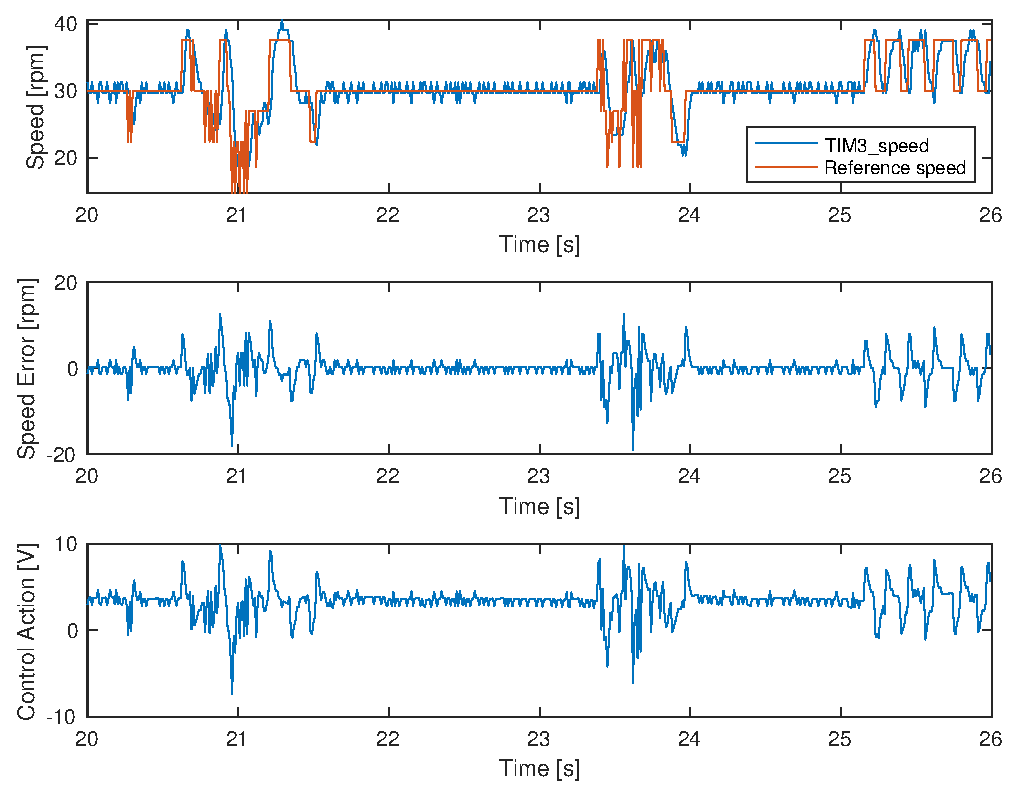
\includegraphics[width=\textwidth]{lab4/figures/wheel_1.eps}
    \end{subfigure}
    
    \vspace{0.5cm} % spazio verticale tra le due figure

    \begin{subfigure}{0.7\textwidth}
        \centering
        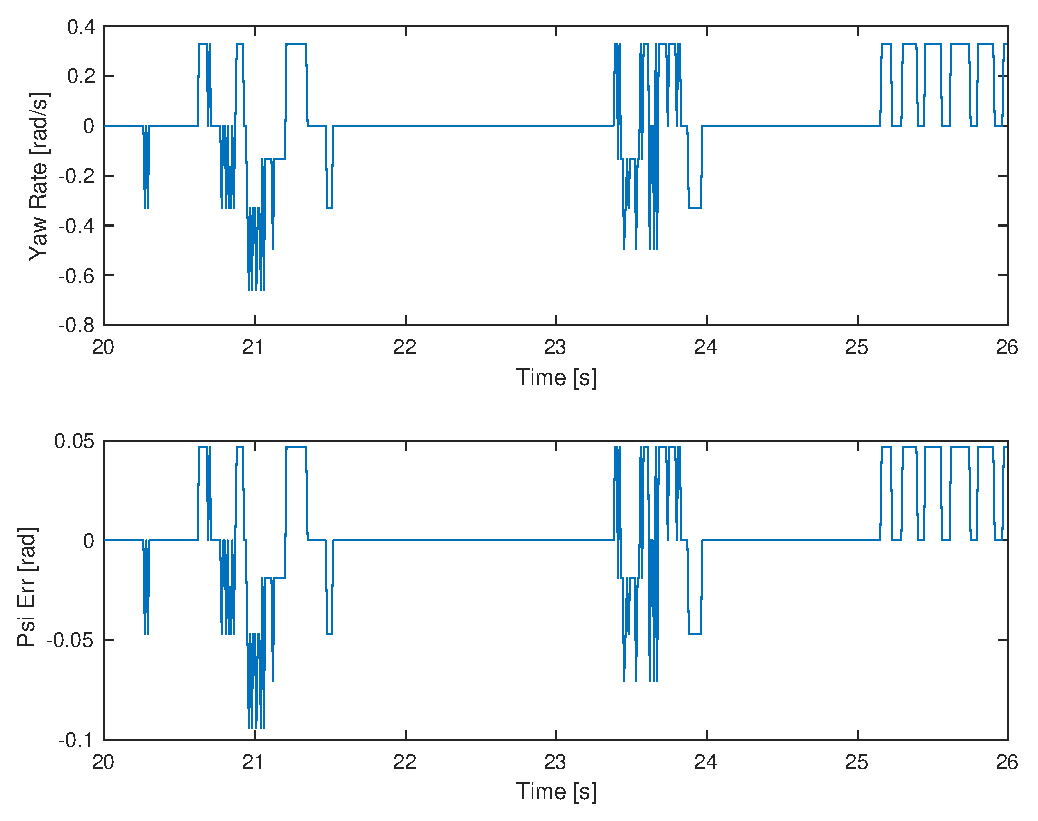
\includegraphics[width=\textwidth]{lab4/figures/yaw_1.eps}
    \end{subfigure}

    \caption{Yaw controller results for wheel 1}
    \label{fig:yaw_controller_results_wheel_1}
\end{figure}

From the first subplot, it is evident that the controller for Wheel 1 is able to track the reference speed with reasonable accuracy, especially during steady-state segments. 
Transient deviations occur when the reference signal changes abruptly, leading to observable overshoots and undershoots. 
These are reflected in the speed error plot, where oscillations are more pronounced in the initial and final parts of the time window.

The third subplot shows the control action in volts. 
The control signal remains mostly within the saturation limits of ±10V, indicating that the controller operates within feasible bounds. 
The presence of sharp control changes suggests that the system is responding to rapid reference changes or disturbances, consistent with what is expected in a dynamic line-following scenario.

The yaw rate plot demonstrates that the robot frequently adjusts its orientation to maintain the desired trajectory, with several peaks and zero-crossings indicating turns or corrections. 
Importantly, the psi error remains mostly bounded within ±0.1 rad, indicating effective heading control throughout the experiment.

\begin{figure}[H]
    \centering
    \begin{subfigure}{0.7\textwidth}
        \centering
        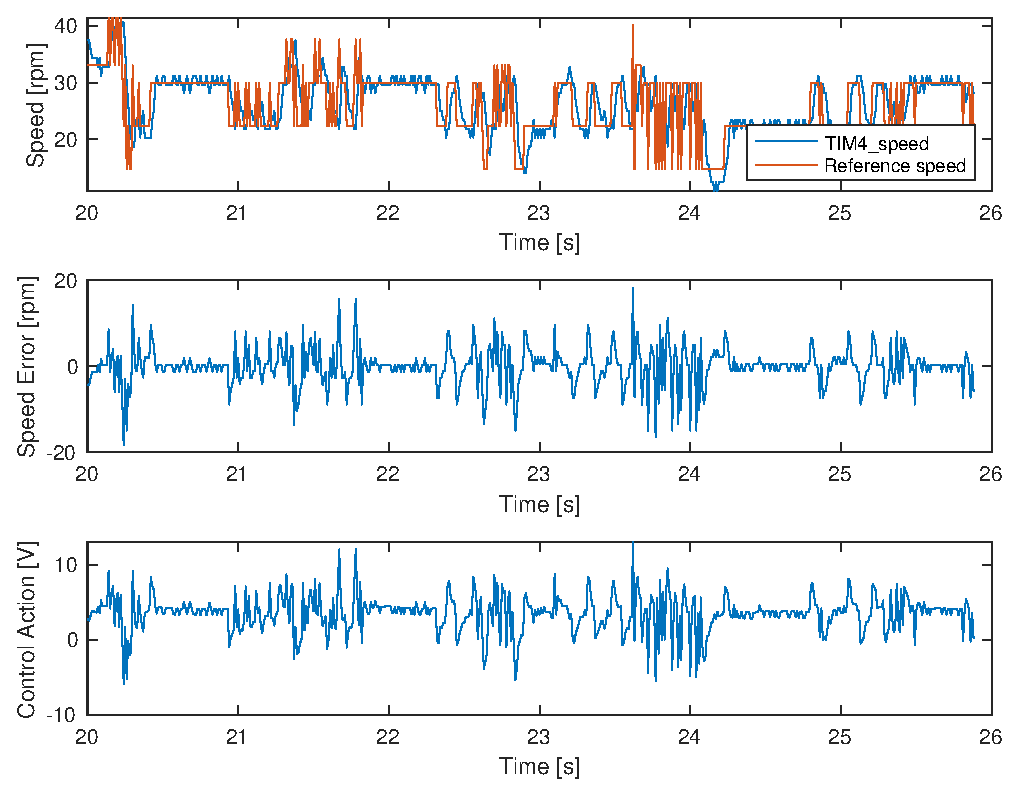
\includegraphics[width=\textwidth]{lab4/figures/wheel_2.eps}
    \end{subfigure}
    
    \vspace{0.5cm} % spazio verticale tra le due figure

    \begin{subfigure}{0.7\textwidth}
        \centering
        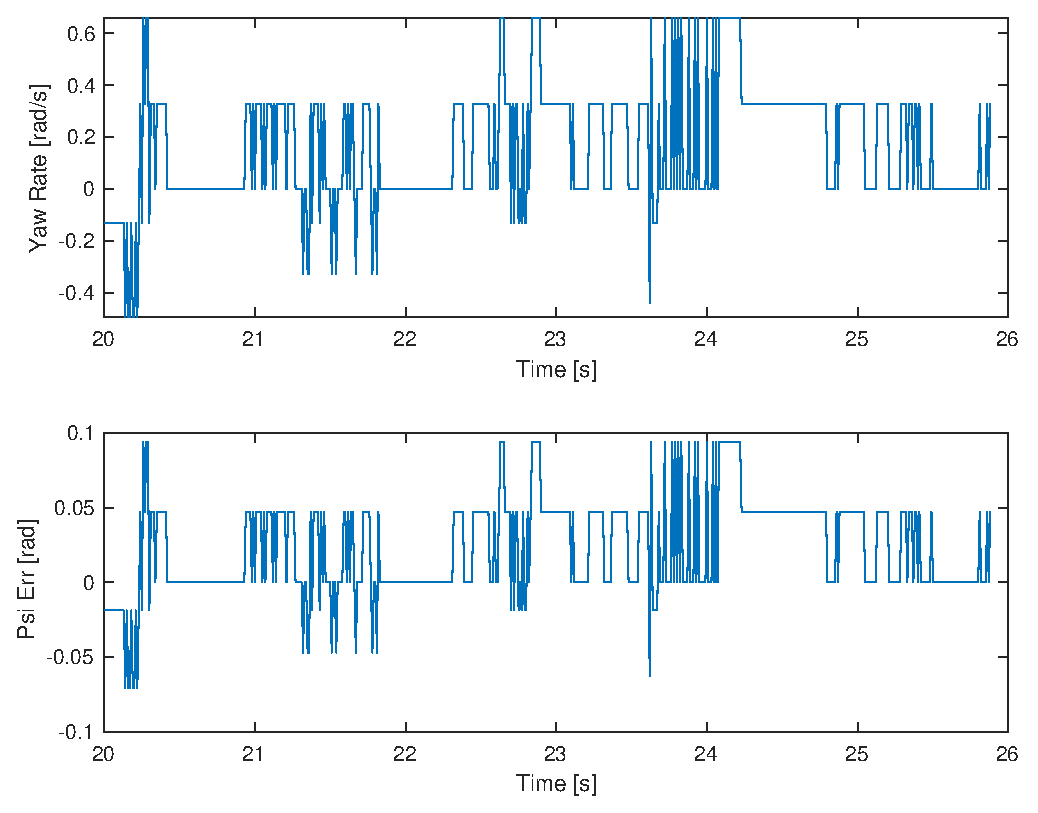
\includegraphics[width=\textwidth]{lab4/figures/yaw_2.eps}
    \end{subfigure}

    \caption{Yaw controller results for wheel 2}
    \label{fig:yaw_controller_results_wheel_2}
\end{figure}

The behavior of Wheel 2 follows a similar trend, although some differences can be observed. 
The reference tracking in the first subplot appears slightly more oscillatory, likely due to asymmetries in the mechanical response or load distribution. 
Moreover, the data collected for Wheel 1 and Wheel 2 corresponds to different simulations (due to the limited capacity of the datalogger), which may explain some of the discrepancies in the speed profiles.
The speed error is larger during some transitions, which translates to more aggressive control actions in the third subplot.

Despite this, the control voltage remains within saturation bounds and demonstrates good responsiveness. 
The yaw rate and psi error plots again confirm that the controller achieves continuous correction of orientation. 
Notably, psi error remains within the same tight bounds observed for Wheel 1, reinforcing the robustness of the overall yaw control strategy.

Overall, the yaw controller successfully maintains trajectory alignment by dynamically adjusting the individual wheel speeds. 
Both wheels contribute to heading correction, and the system demonstrates good performance in terms of responsiveness, error containment, and control effort. 
These results validate the effectiveness of the implemented controller in enabling stable and accurate line following under varying speed references and disturbances.